\documentclass{lab}

\renewcommand{\AA}{\ensuremath{\mathring{A}}}

\begin{document}

\labtitle{5.4.1}{Определение энергии $ \alpha $-частиц по величине их пробега в воздухе}{14~ноября~2019~г.}{21~ноября~2019~г.}

\section*{Постановка эксперимента}

\begin{quote}
	\textbf{{\normalsize Цель работы: }}измерить пробег $ \alpha $-частиц в воздухе двумя способами: торцевым счетчиком Гейгера и ионизацонной камерой. Определить энергию частиц.
\end{quote}
	
Связь между энергией $ \alpha $-частицы и периодом полураспада радиоактивного ядра описывается формулой:
\begin{equation}
\ln\left( T_{1/2} \right) = \dfrac{a}{\sqrt{E}} + b
\end{equation}
Формула ионизационных потерь нерелятивистской тяжелой заряженной частицы имеет вид:
\begin{equation}
\left( \dfrac{dE}{dx} \right) \approx 2\pi \dfrac{e^4z^2}{mv^2}\cdot nZ \cdot \ln\left( \dfrac{2mv^2}{\bar{I}} \right)
\end{equation}

\section*{Экспериментальная установка}

	Схемы установок, используемых в работе, показаны на рисунке \ref{1}.
	
	\begin{figure} [h!]
		\centering
		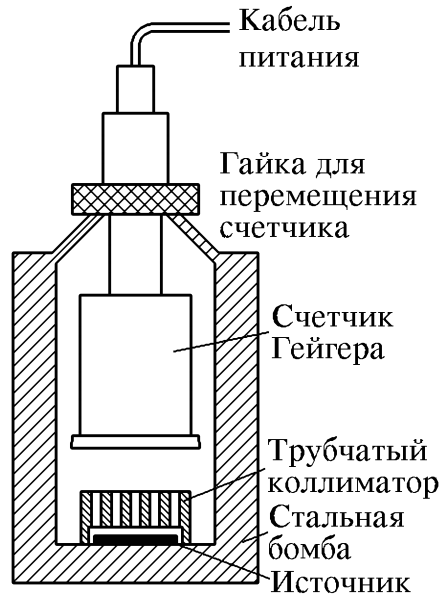
\includegraphics[width=0.35\linewidth]{1}
		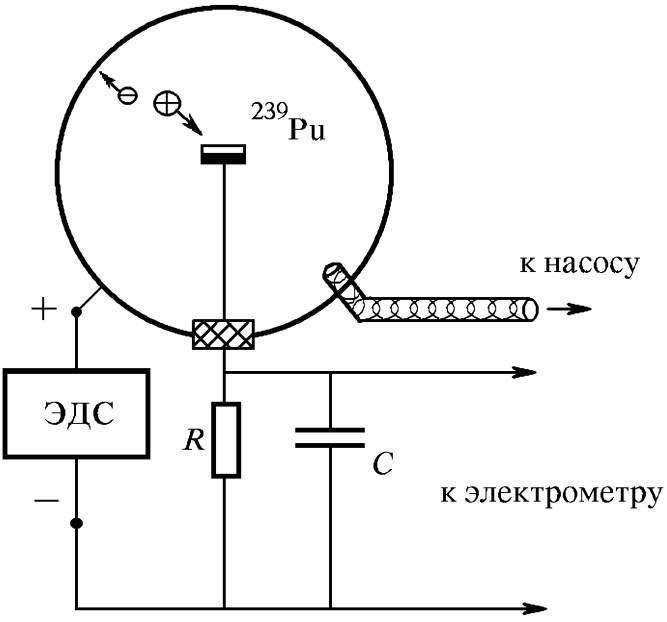
\includegraphics[width=0.5\linewidth]{2}
		\caption{Схемы установок для исследования длины пробега $ \alpha $-частиц.}
		\label{1}
	\end{figure}


\newpage

\section*{Выполнение работы}
\begin{gather*}
	p_{атм} = 757~mm~Hg\\
	I_0 = 4~пА\\
	I_{745} = 16~пА
\end{gather*}
\subsection*{Счетчик Гейгера}
\begin{enumerate}
\item
Проделаем измерения:
\begin{table}[H]
	\centering
	\begin{tabular}{|cccc|}
		\hline
		$x,~мм$ & $t,~с$ & $N,~шт$ & $N/t,~с^{-1}$ \\ \hline
		10&	60	&	816	&13.6	\\
		14&	60	&	869	&14.5	\\
		16&	60	&	837	&14.0	\\
		17&	60	&	658	&11.0	\\
		18&	60	&	374	&6.3	\\
		19&	60	&	55	&0.9	\\
		20&	60	&	15	&0.2	\\
		24&	63	&	18	&0.3	\\
		28&	60	&	9	&0.2	\\
		\hline
		
	\end{tabular}
	\label{tab1}
\end{table}

\item 
График зависимости реагирования на частицы от расстояния до счетчика от излучателя:
\begin{figure}[H]
	\centering
	\begin{tikzpicture}
	
	\pgfplotstableread{
		X	    Y			x-err		y-err
10	13.6		0.3	0.2
14	14.53177258	0.3	0.2
16	13.95		0.3	0.2
17	11.00334448	0.3	0.2
18	6.254180602	0.3	0.2
19	0.922818792	0.3	0.2
20	0.249584027	0.3	0.2
24	0.285714286	0.3	0.2
28	0.151260504	0.3	0.2

	}{\mytable}
	
	\begin{axis}[
	width = 0.75\textwidth,
	grid = major,
	xlabel = $ x\text{,}~\text{мм} $,
	ylabel = $ N/t\text{,}~\text{c}^{-1} $,
	ymin = 0,
	ymax = 15,
	xmin = 8,
	xmax = 30
	]
	
	
	\addplot[
	only marks,
	color = red,
	mark = *,
	error bars/.cd,
	x dir = both,
	x explicit,
	y dir = both,
	y explicit
	]
	table[
	x error = x-err,
	y error = y-err
	] {\mytable};
	
%	\addplot[
%	mark = none,
%	color = red
%	]
%	table[
%	y = {create col/linear regression={y=Y}}
%	] % compute a linear regression from the
%	{\mytable};
	
	\end{axis}
	\end{tikzpicture}
	\caption{Счетчик Гейгера}
	\label{graph1}
\end{figure}

\item 
Длина пробега $ \alpha $-частицы с помощью экстраполяции: $ R = 19 \pm 0.5 ~мм $.

\end{enumerate}

\subsection*{Ионизационная камера}

\begin{enumerate}

\item
Зависимость тока от давления в ионизационной камере:
\begin{table}[H]
	\centering
	\begin{tabular}{|cc|cc|}
		\hline
		$ P,~торр $ & $ I,~пА $ & $ P,~торр $ & $ I,~пА $ \\ \hline
		740&	23	&350	&700\\
		725&	38	&330	&742\\
		700&	75	&310	&783\\
		670&	124	&290	&828\\
		650&	155	&270	&877\\
		630&	185	&250	&920\\
		610&	220	&230	&955\\
		590&	252	&210	&993\\
		570&	283	&190	&1005\\
		550&	319	&170	&1016\\
		530&	357	&150	&1019\\
		510&	393	&130	&1012\\
		490&	430	&110	&1005\\
		470&	463	&90		&1003\\
		450&	500	&70		&1000\\
		430&	541	&50		&993\\
		410&	585	&30		&987\\
		390&	620	&10		&981\\
		370&	663	&0		&977\\
		\hline
		
	\end{tabular}
	\label{tab2}
\end{table}

\newpage
\item
График зависимости тока от давления в ионизационной камере:

\begin{figure}[H]
	\centering
	\begin{tikzpicture}
	
	\pgfplotstableread{
		X	    Y			x-err		y-err
		740	23	5	1
		725	38	5	1
		700	75	5	1
		670	124	5	1
		650	155	5	1
		630	185	5	1
		610	220	5	1
		590	252	5	1
		570	283	5	1
		550	319	5	1
		530	357	5	1
		510	393	5	1
		490	430	5	1
		470	463	5	1
		450	500	5	1
		430	541	5	1
		410	585	5	1
		390	620	5	1
		370	663	5	1
		350	700	5	1
		330	742	5	1
		310	783	5	1
		290	828	5	1
		270	877	5	1
		250	920	5	1
		230	955	5	1
		210	993	5	1
		190	1005	5	1
		170	1016	5	1
		150	1019	5	1
		130	1012	5	1
		110	1005	5	1
		90	1003	5	1
		70	1000	5	1
		50	993	5	1
		30	987	5	1
		10	981	5	1
		0	977	5	1
		
		
	}{\mytable}
	
	\begin{axis}[
	width = 0.75\textwidth,
	grid = major,
	xlabel = $ P\text{,}~\text{торр} $,
	ylabel = $ I\text{,}~\text{пА} $,
	ymin = 0,
	ymax = 1200,
	xmin = 0,
	xmax = 800
	]
	
	
	\addplot[
	only marks,
	color = red,
	mark = *,
	error bars/.cd,
	x dir = both,
	x explicit,
	y dir = both,
	y explicit
	]
	table[
	x error = x-err,
	y error = y-err
	] {\mytable};

	%	\addplot[
	%	mark = none,
	%	color = red
	%	]
	%	table[
	%	y = {create col/linear regression={y=Y}}
	%	] % compute a linear regression from the
	%	{\mytable};
	
	\end{axis}
	\end{tikzpicture}
	\caption{Ионизационная камера}
	\label{graph2}
\end{figure}

\item 
\begin{gather*}
	R = \dfrac{P_0}{P_{атм}} (D_2 - D_1)\\
	D_1 = 100~мм~~~~~D_2 = 5~мм\\
	P_0 = 587~торр\\
	R = 19 \pm 0.3 ~мм
\end{gather*}

\item 
\begin{gather*}
	R(T,P) = \dfrac{T_0}{T} \dfrac{P_0}{P} \Delta D\\
	R(15^(\circ), 760~торр) = \dfrac{297}{288} \dfrac{587}{760} = 20 \pm 0.3~мм
\end{gather*}

\item 
Определение энергии частицы:
\begin{equation}
E = \left( \dfrac{R}{0.32} \right) ^{2/3} = 12.3 \pm 0.5~МэВ
\end{equation}

\end{enumerate}

\subsection*{Итоги}

Средняя длина пробега $ \alpha $-частиц: $ R = 19.0 \pm 0.5 ~ мм$ при нормальных условиях.

\end{document}